\chapter{Introduction}\label{chap:chapter1}

The work presented in this thesis is part of an industry-linked PhD under the Centre for Transforming Maintenance Through Data Science (CTMTDS), a centre comprised of both academic and industry partners. One of the Centre's goals is to develop methods that support reliability engineers in managing uncertainty during the maintenance decision making process---how and when they should maintain an asset based on their understanding of the asset, the available data, and what this data tells them about the current condition of the asset. As part of the industry-linked PhD, I spent 900 hours working on industry placement projects between two different industry partners to define research topics that are not only novel in an academic sense but also useful for applied problems in reliability that are faced by practitioners when making maintenance decisions in the mining and mineral processing industry.

From my placement time, it was apparent that there was a disconnect between the reliability modelling literature and the methods used by reliability practitioners in the mining and mineral processing industry---a theory-practice gap. There are many well-established models for reliability data, such as the Weibull distribution \citep{weibull1951} for lifetime data or stochastic process models for degradation data. There is also a desire by mine, processing plant, and refinery operators to use these models since once an asset is put into service, completely new information becomes available in the form of infield reliability data, which can be utilised so that operators can make better maintenance decisions based on the specific reliability characteristics of their assets, rather than estimates from the manufacturer \citep{jardine2013}. However, these in-field data are typically noisy, messy, incomplete and uncertain as a result of unique observational processes that need their own sophisticated modelling approaches before reliability practitioners in the mining and mineral processing industry can take advantage of the well-established reliability models in the literature. Two examples of issues confronting reliability engineers that I tackle in this thesis are 1) obtaining sensible estimates of lifetime distributions when lifetime data are heavily censored and truncated due to the pre-emptive replacements of assets and the way in which data is recorded, and 2) forecasting complex degradation processes with noisy and sparsely observed condition monitoring data. In this thesis, I develop novel extensions of some of the well-established reliability methods through the Bayesian model building approach \citep{gelman_workflow_2020} and demonstrate how they can be applied to observational industry data sets from overland iron ore conveyors provided by the Centre's industry partners.

The Bayesian paradigm became the basis of this thesis because Bayesian methods provide a formal structure to build complicated models and incorporate multiple sources of information, such as domain expert knowledge \citep{Meeker2022}. Furthermore, the resulting full posterior distribution obtained from Bayesian analysis allows us to easily produce estimates and uncertainty intervals of complicated functions of the model parameters \citep{Meeker2022}, which is extremely useful for propagating uncertainty through a decision-making process. While there is a well-developed subfield of Bayesian analysis in the reliability literature \citep{hamada_2008, Meeker2022}, the Bayesian framework is underutilised in industry. This underutilisation is most likely because, for most cases, inference must be obtained through Monte Carlo simulation, and in the past, this has meant constructing Markov Chain Monte Carlo (MCMC) algorithms manually. However, the recent increase in popularity of Bayesian methods is due to the development of flexible and accessible probabilistic programming languages such as BUGS \citep{lunn2012}, JAGS \citep{plummer2003} and Stan \citep{Stan2022}, which in many cases alleviate the analyst from the need to construct bespoke MCMC algorithms. The result is a newfound ability to fit and explore complex models relatively quickly and simply.

To harness these new aspects of statistical modelling more effectively, the applied Bayesian statistical community has started to develop a more rigorous workflow for building, fitting, checking, and comparing Bayesian models \citep{gelman_workflow_2020}. Throughout this thesis, I emphasise the components of this workflow and demonstrate them in a reliability setting. In doing so, I hope this thesis may also be used as a template for how to carry out and report the results of Bayesian analyses for reliability and maintenance problems in the field.

The remainder of this chapter provides a background to the rest of the Thesis. First, in Sec.~\ref{sec:decisions}, I provide some context around maintenance decision-making in the mining and mineral processing industry. Then, Sec.~\ref{sec:reliability}, I give a high-level overview of reliability modelling and how it informs maintenance decisions. Section~\ref{sec:industry-data} describes two industry data sets that I use as case studies. Section~\ref{sec:Bayesian-methods} outlines Bayesian methods and the key components of the Bayesian model-building workflow, which will be a strong thread throughout the remainder of the thesis. Finally, in Sec.~\ref{sec:thesis-structure}, I lay out the structure of the thesis.

\section{Maintenance decision making}
\label{sec:decisions}

The maintenance of an asset can be considered as ``all activities aimed at keeping an [asset] in, or restoring it to, the physical state considered necessary for the fulfilment of its production function'' \citep{geraerds1985}. In other words, the main objective of maintenance actions is to fix/replace an asset's components to ensure that it can perform its desired duty at an acceptable level of performance. In this context, the only consideration when deciding when to maintain the asset is whether or not the asset is performing its duty at an acceptable level. However, in reality, the maintenance of any single asset exists in the much larger context of a company \citep{jardine2013}. There are finite resources, budget, and time that can be allocated to the maintenance of any specific asset, and some assets are more critical to production than others. This `big picture' management of an asset's maintenance is what we refer to as asset health management. It is in this bigger context that reliability engineers and planners must make their decisions about how and when to maintain an asset. Asset health management requires foresight, planning, and---most importantly---risk management.

Maintenance strategies help to allocate resources and plan maintenance schedules ahead of time. There are three general strategies: reactive, preventative, and predictive maintenance \citep{jardine2013}. I provide a more detailed overview of these strategies below, but first, note that an asset can have different strategies for its different components, and typically, the choice of strategy is dictated by how critical the component is, how expensive it is, and what type of data we can collect. But even with a maintenance strategy, once an asset is put into service, we start to gather new reliability or condition monitoring data that can be used to refine/inform the maintenance strategy. For instance, Chap.~\ref{chap:chapter3} uses failure time data to inform the timing of bulk-replacements in a preventative maintenance strategy.

\subsubsection*{Reactive vs Preventative vs Condition-based maintenance strategy}

The simplest replacement strategy is a reactive maintenance strategy whereby components are only replaced once they fail \citep{heng2009}. Reactive strategies are used mostly for non-critical components. They are not typically used for mechanical components in mining because the cost due to lost production when an asset must be replaced unexpectedly is orders of magnitude greater than the cost of planned maintenance. On the other hand, a preventative replacement strategy is when components are replaced pre-emptively after a designated period of time or operation. This proactive approach to maintenance is suitable for cheap components whose reliability decreases with time, i.e., components that wear out (most mechanical components). A disadvantage of preventative maintenance is that it can result in overmanning assets (replacing components too frequently when they still have remaining useful life), which is a waste of money and resources. If a component is costly and critical, and it is possible to monitor its condition, then a condition-based maintenance strategy should be used. Condition-based maintenance balances using as much of the component's useful life as possible with the reduced risk of lost production by monitoring the degradation of a component and replacing it when it gets to a predetermined, unacceptable level.

There are obvious ways in which statistical modelling can inform preventative and condition-based strategies. Implementing a preventative replacement strategy requires choosing a pre-emptive time to replace the component. The better that the choice balances the cost of maintenance with the cost of unplanned failure, the better the strategy will perform. A component's specific environmental and operating conditions affect its reliability \citep{Meeker2022}. So, if it is possible to use data to `tune' the replacement time to the component's reliability under the specific operating conditions, then the preventative policy will be more successful than one where the manufacturer's default recommendations are used. Condition-based strategies, on the other hand, are more useful if we can forecast the degradation through time to predict the failure time (or remaining useful life) of the component. More detailed and accurate forecasts will result in better maintenance plans and reduce the risk of an unexpected failure. In both cases, the more accurately we can estimate the reliability quantities, the better the strategies will perform.

\section{Reliability modelling}
\label{sec:reliability}

In the engineering context, reliability is the ``ability of an item to perform a required function under given conditions for a given time interval'' \citep{ISO_14224_2016}. This definition is very closely tied to the definition of maintenance actions in Section~\ref{sec:decisions}; maintenance actions are to ensure reliability. In the reliability modelling context, the definition of reliability is slightly different. It is the ``probability for an item to perform a required function under given conditions over a given time interval $(0, t)$'' \citep{ISO_12489_2013}. In other words, it quantifies the engineering definition of reliability as a probability that a unit will not fail before $t$, that is, $\text{Pr}\left[T > t\right]$, where $T$ is the time of failure. Here, time $t$ can be calendar time, operating time, or some other exposure, such as loading cycles, distance travelled, or throughput \citep{lee2006}.

The modelling definition of reliability focuses on binary outcomes (i.e. success/failure data) for a given time interval \citep{hamada_2008}. But typically, we have more detail in data and instead want to estimate the reliability at all values of $t = [0, \infty)$. This representation is the reliability function, $R(t)$ (also called the survival function, $S(t)$). Reliability can alternatively be expressed as the complement of the reliability function, $\text{Pr}\left[T \le t\right]$, which is the cumulative failure time distribution, $F(t)$ \citep{Meeker2022}. Reliability analysis aims to estimate these functions from data. Two general approaches are taken, depending on the type of observations available: lifetime modelling (also referred to as failure time models) and degradation models (sometimes referred to as repeated measures degradation models).

\paragraph*{Lifetime modelling} 

The most common form of reliability data are lifetime data. These are the recorded installation and failure times of units in operation. Lifetime modelling, therefore, aims to estimate the failure time distribution from lifetime data. These lifetime data can come from repeated failures of an asset or the lifetimes of a population of assets. The estimated failure time distribution from lifetime analysis allows the analyst to make general statements about the reliability of a population conditional on some exposure time $t$ and sometimes on covariates \citep{moore2016}. However, it is common for reliability datasets to be limited in size or the number of observed failures \citep{Meeker2022}. For example, a particular asset may only have a small number of failures, or in a population of highly reliable assets, only a few may fail over the period of observation. In these cases, the data are not very informative of the parameters in a lifetime model. To combat a lack of information, the analyst can either supplement the analysis with other sources of information (which we elaborate on in Part~\ref{part:one}) or use a degradation model if they have access to measurements of the degradation process that drives failure (the focus of Part~\ref{part:two}).

\paragraph*{Degradation modelling} 

To use an example from \citet{Meeker2022}, consider the case that in a lifetime dataset, only two out of one hundred units fail. In this case, the ninety-eight units that did not fail provide no information about how close they were to failure. If, in addition, there are repeated measurements of the level of the degradation that drives the failure, then degradation analysis allows us to incorporate how close the other ninety-eight units were to failing into the analysis and more precisely estimate the failure time distribution. In fact, degradation modelling can be used to derive failure time distributions if there are no failures or even for a single unit that has not yet failed (Part~\ref{part:two}). The connection between degradation models and failure time distribution is well explored \citep{lu1996,bae2007,Meeker2022,lawless2004}, and the connection is typically made using, not catastrophic failure, but soft failure.

Soft failure is defined by a predetermined threshold of degradation, compared to hard failures, which occur when the component can no longer operate \citep{hamada_2008}. Hard failures are more uncertain in nature, since the level of degradation is only indicative of when the component will catastrophically fail---e.g. the catastrophic failure of a steel beam with a crack in it is both a function of the cracks length and the random load applied to the beam---making them more risky, hence why soft failure is often used. However, regardless of whether a soft or hard failure definition is used, when the failure time distribution is derived from a degradation model, it is important to note that the distribution is conditional on the particular degradation failure mode we are modelling.

Statistical degradation models can be divided into general path models and stochastic process models \citep{pandey2006, si2011}. General path models assign a functional and/or empirical form to the degradation path of a unit, typically a theoretically motivated function such as in \citet{robinson2000}. This method assumes that the functional form can sufficiently represent the underlying degradation and that measurement error can completely account for any deviations in measurements from this fixed path. Heterogeneity between units can be added through regression/random effects \citep{robinson2000}. On the other hand, stochastic processes do not assume a fixed path \citep{pandey2006}. In stochastic processes, the jumps in degradation are modelled as random variables, meaning that they account for random variation in the degradation process over time. The stochastic process model I focus on is the Gamma process, as in \citet{lawless2004}. A limited comparison of the two methods is made in \citet{ye2015}; however, no comprehensive comparisons have been explored.

\section{Industry Examples}
\label{sec:industry-data}

In this thesis, I show two examples of industry problems. Both problems relate to the components of an overland iron ore conveyor. One example is a preventative maintenance problem, and the other is a condition-based one. In Part~\ref{part:one} of the thesis, I look at the preventative replacement of idlers, whereas in Part~\ref{part:two} I focus on forecasting the degradation of a conveyor's belting to inform condition-based decisions. The two components are shown in Fig.~\ref{fig:belt_and_frame}.

\begin{figure}[tbp]
  \centering
  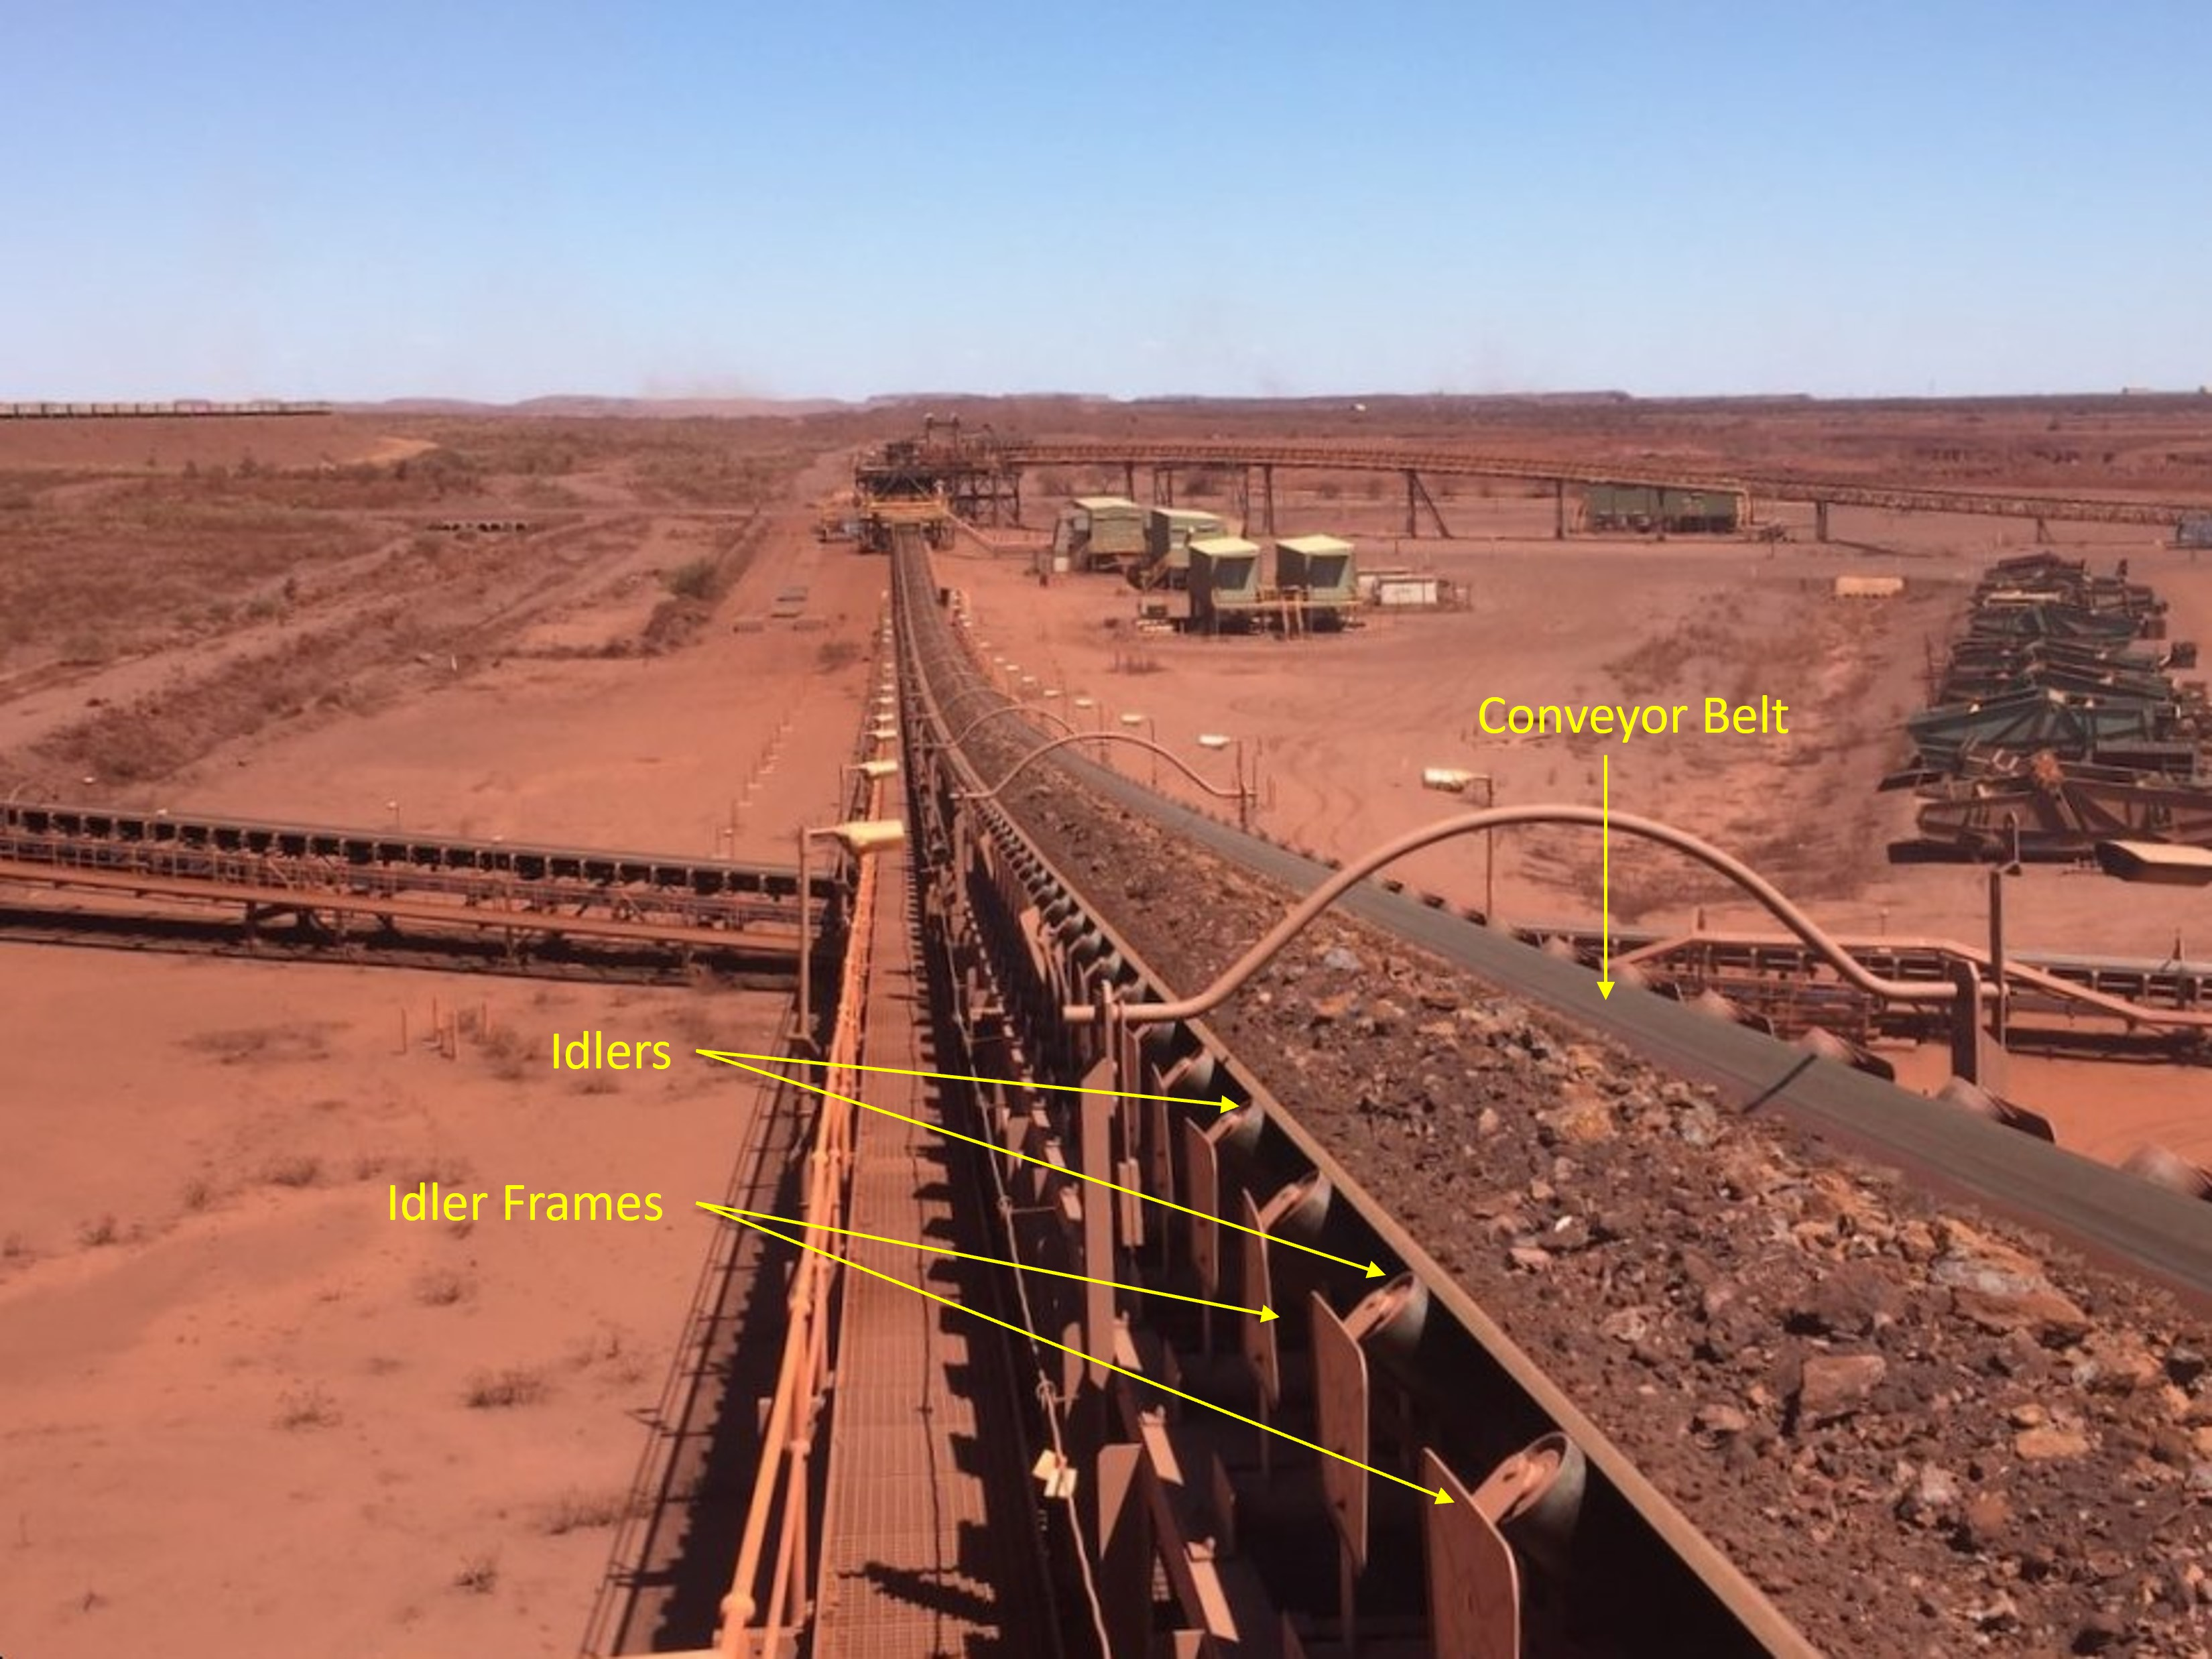
\includegraphics[width=0.95\textwidth]{./figures/ch-1/cvr_example_edit_annotation.jpg}
  \caption{An annotated image of an overland iron ore conveyor \citep{australianmining2020} showing the belting, idlers, and idler frames.}
  \label{fig:belt_and_frame}
\end{figure}

\paragraph*{Idlers}

Idlers (sometimes called rollers) support the weight of the belt and ore. They are relatively cheap components, and there can be hundreds or thousands of them on a single conveyor. Idlers are organised in frames, usually consisting of three idlers: one central idler directly under the belt and two wing idlers supporting the sides of the belt to create the cupped shape. The idlers and idler frames are shown in Fig.~\ref{fig:belt_and_frame}. Idlers are mechanical components and, therefore, wear out with operation. When an idler fails, it does not cause a direct impact on production; however, failed idlers can damage the belt, and damage to the belt results in major downtime. Therefore, if an idler fails in a way that threatens to damage the belt, it must be replaced as soon as possible, causing an unplanned maintenance event. Reliability engineers need to manage the replacement of the idlers to minimise the risk of them failing and damaging the belt while simultaneously minimising the maintenance cost. It is not yet financially viable to monitor the condition of all idlers on a single conveyor, let alone all conveyors on a mine site. Therefore, a preventative maintenance strategy is used.

\begin{figure}[tbp]
  \centering
  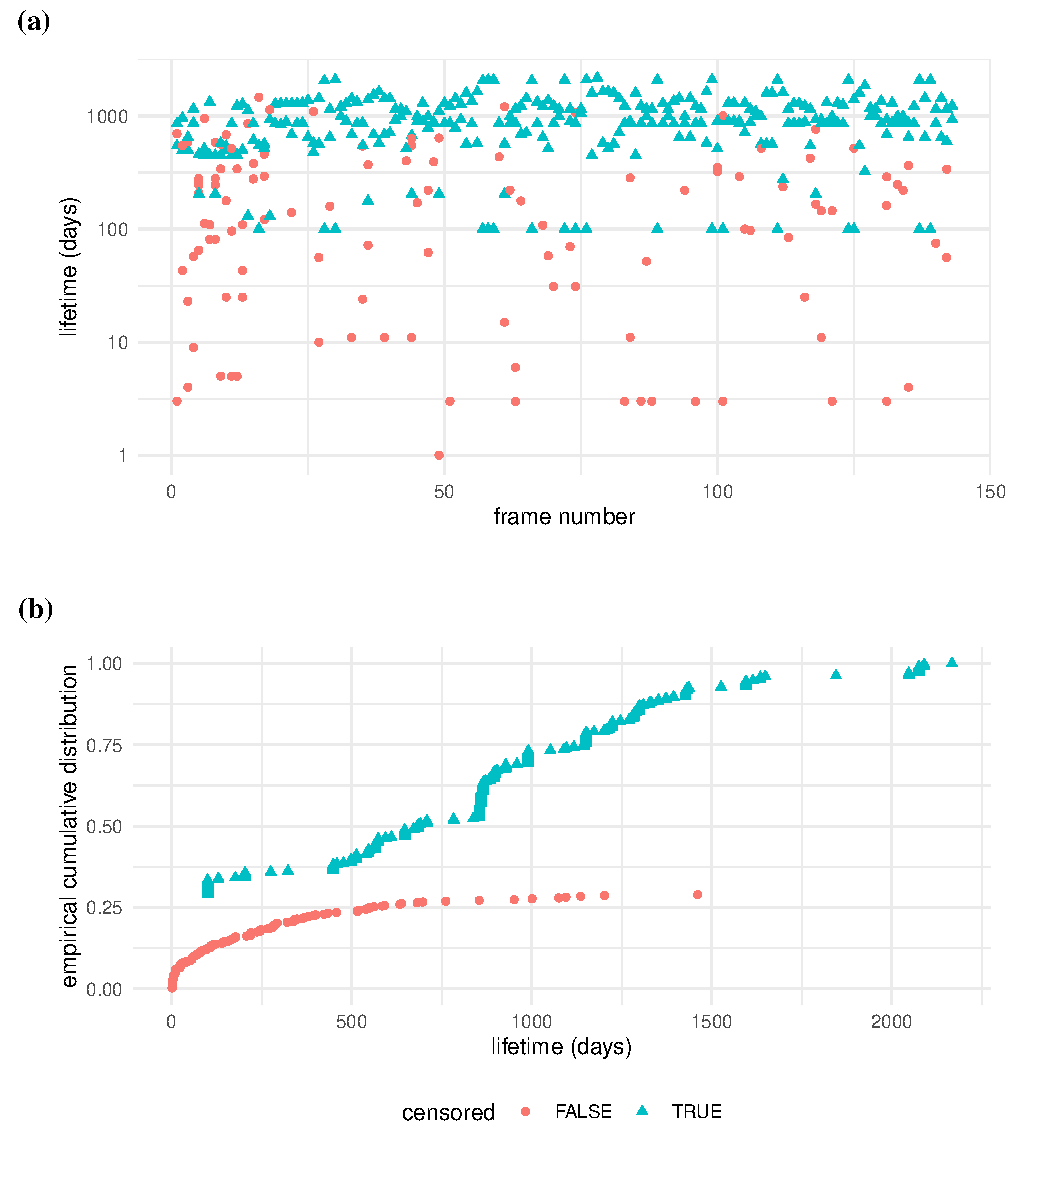
\includegraphics[width=0.95\textwidth]{./figures/ch-1/idler_data_desc.pdf}
  \caption{The idler frame lifetime dataset. (a) shows the lifetimes on a log scale for each frame plotted along the length of the conveyor and (b) the empirical cumulative distribution function (eCDF) of lifetimes. The blue points show the lifetimes that were only partially observed.}
  \label{fig:idler-data}
\end{figure}

The survival data of idler frames I use in this thesis, derived from their installation and replacement times, can be used to inform the preventative maintenance strategy. Unfortunately, the failure data is only reliably recorded down to the frame number level, not the position of the idler in the frame. However, when one of the idlers in a frame fails, usually all the idlers in that frame are replaced, meaning that we can model the reliability of the idler frames to inform the preventative maintenance strategy. The data set is shown in Fig.~\ref{fig:idler-data}~(a). The figure shows the frame lifetimes for a single overland conveyor over six years. Because idlers are long-lasting components and also because they are preventatively replaced, there are many cases where we do not observe the entire lifetime of an idler, either because it had not failed by the time we stopped observing it, it was pre-emptively replaced, or it was in operation before we started reliably capturing failure and installation data. These partially observed lifetimes are censored and/or truncated lifetimes and are shown in blue in Fig.~\ref{fig:idler-data}~(a). I discuss censoring and truncation in more detail in Part~\ref{part:one} of the thesis. Figure~\ref{fig:idler-data}~(b) shows the observed and partially observed lifetimes plotted cumulatively. In the ordered plot, we can see that many of the shorter lifetimes are fully observed, while most long lifetimes are obscured by censoring.

\paragraph*{Belt}

The belt of an overland conveyor is much more costly to replace, both in terms of time and money. Furthermore, if the belt fails, then major downtime is inevitable. Over time, the constant loading of ore onto the belt wears away a protective topcoat of rubber, exposing the structural components of the belt to the risk of being damaged by the ore. To assess the structural integrity of the belt, engineers stop the belt occasionally to take ultrasonic-thickness (UT) measurements of the topcoat and make sure that it is thick enough to provide adequate protection. An example of the UT data is shown in Fig.~\ref{fig:belt_wear_ut}.

Engineers use these UT measurements to estimate the soft failure time of the belt and plan its replacement, i.e. forecast when the top coat will no longer be thick enough to protect the belt. However, forecasting the wear of the belt to inform replacement decisions requires principled statistical modelling to properly quantify the many different sources of uncertainty, which can be done in the Bayesian framework.

\begin{figure}[tbp]
  \centering
  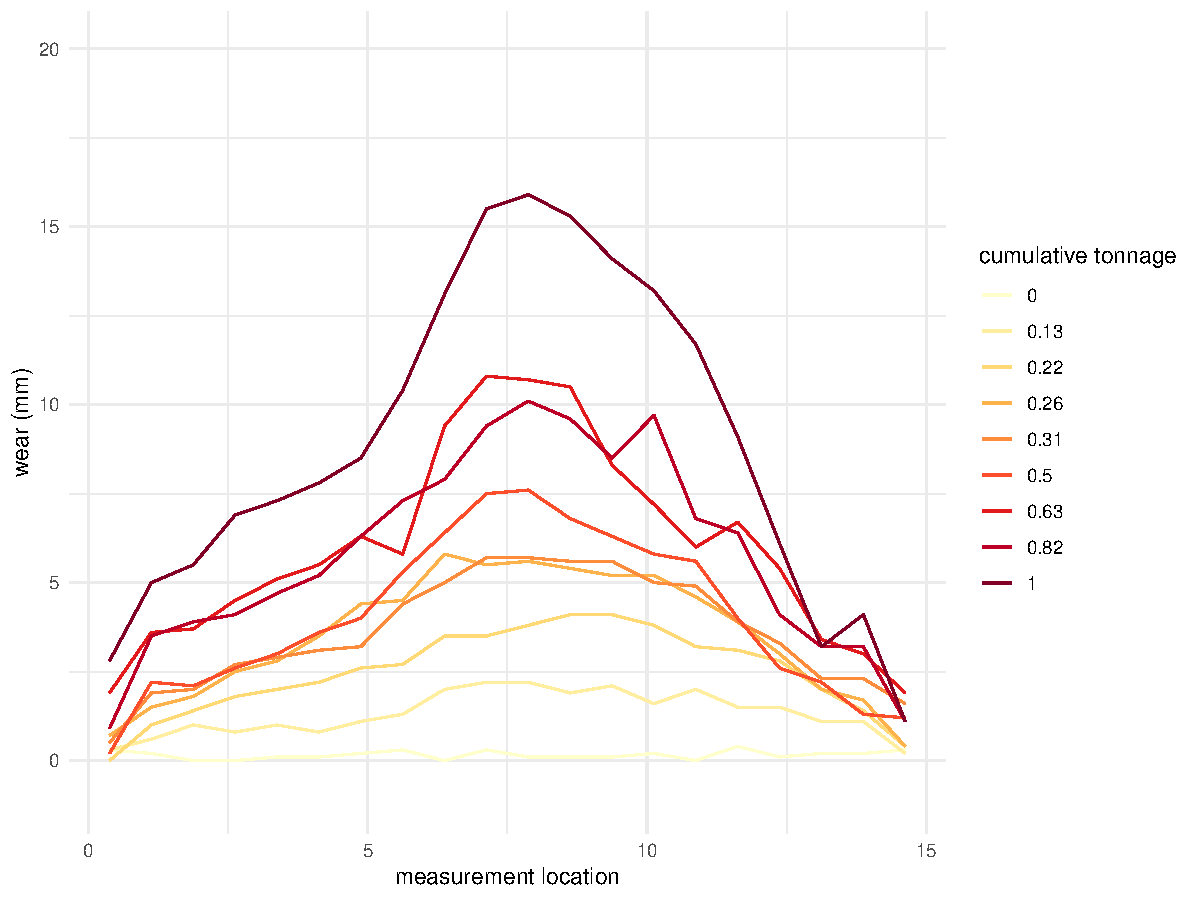
\includegraphics[width=0.95\textwidth]{./figures/ch-1/belt_wear_ut.pdf}
  \caption{The conveyor belt wear degradation dataset. The lines show the wearing surface across the width of a conveyor's belt. The colour scale indicates the cumulative tonnes (standardised) or iron ore throughput that the belt has moved (effectively the utilisation time).}
  \label{fig:belt_wear_ut}
\end{figure}

\section{Bayesian reliability modelling}
\label{sec:Bayesian-methods}

In the Bayesian statistical framework, probabilities are subjective statements about our uncertainty. In a Bayesian analysis, we aim to construct probability statements about parameters of interest, $\theta$, conditioned on the data $y$ and (implicitly) on the values of covariates \citep{BDA2020}. That is, we wish to obtain $p(\theta|y)$, known as the posterior distribution. To do this, Bayesian inference relies on Bayes rule,
\begin{equation}
  p(\theta|y) = \frac{p(y|\theta)p(\theta)}{p(y)},
\end{equation}
where $p(y|\theta)$ is the likelihood of the data conditional on $\theta$, $p(y)$ is the marginal distribution of the data, and $p(\theta)$ is the prior distribution of the parameters. The prior distribution encodes our belief about the parameters before observing the data and, therefore, encodes any additional information that we may have about the phenomenon we are modelling, either from historical data or domain expertise. Alternatively, we can write the un-normalised posterior as
\begin{equation}
  p(\theta|y) \propto p(y|\theta)p(\theta).
\end{equation}

In practice, however, the posterior distribution is rarely available in closed form, and we need to simulate draws from the posterior distribution using Markov chain Monte-Carlo methods to perform inference. There are several powerful and flexible probabilistic programming languages, such as Stan \citep{Stan2022}, which allow us to easily implement MCMC algorithms for complex model structures.

\paragraph*{Bayesian workflow} \label{sec:bayesian-background}

Surrounding Bayesian inference is a larger workflow of good statistical practice. Just as there is good practice for statistical modelling, the applied Bayesian community has developed its own workflow tailored to the specifics of Bayesian analysis \citep{gelman_workflow_2020}, the main components of which focus on model construction, drawing from the posterior using MCMC methods and diagnosing issues with computation, sense checking the model with simulated data, evaluating and using the posterior distribution, and comparing and expanding models. Here, I give a very high-level overview of the components in the workflow most relevant to this thesis. See \citet{gelman_workflow_2020} for an in-depth description of a Bayesian workflow. The components of this workflow that I use within this thesis are conditional modelling, prior predictive checking, sampling and diagnostics, posterior predictive checking and posterior inference, and model comparison.

\paragraph*{Model specification}

The first step of any Bayesian analysis is to postulate a joint probability distribution of the model components. For complicated processes, this first step can be simplified by using a Bayesian Hierarchical (multi-level) Modelling approach, which uses the fundamental notion of the \textit{the chain rule}, $p(A, B, C) = p(A|B, C) p(B|C) p(C)$, to decompose a complicated joint probability into a sequence of simpler conditional probabilities \citep[p.~13]{wikle_2019}. \citet{Berliner_1996} proposed Bayesian Hierarchical Modelling (BHM) as a way of studying an underlying latent process by breaking the joint probability of the data, process, and parameters down into three sub-models:
\begin{align*}
 p(\text{data}, \text{process}, \text{parameter}) = & p(\text{data}| \text{process}, \text{parameter}) && \text{data model} \\
 & p(\text{process}| \text{parameter}) && \text{process model} \\
 & p(\text{parameter}). && \text{parameter model}
\end{align*}
The first level is the data model, $p(\text{data} | \text{process}, \text{parameter})$, which describes the observation process. The second level in the hierarchy is the process model, $p(\mbox{process} | \text{parameter})$. It describes the underlying process that is of scientific interest. The third level in the hierarchy, $p(\text{parameter})$, is the parameter model, and, in a Bayesian setting, refers to the prior distribution. Each of these different levels in the hierarchy can also comprise smaller constituent conditional models. \citet{cressie_2011} advocate using the BHM approach for studying underlying latent spatial and spatio-temporal processes, but the same general approach is used to formulate models for nested data structures under the term multi-level modelling \citep{BDA2020}. 

In the last level of this hierarchical structure, the prior distribution summarizes any \textit{a priori} beliefs the analyst has about the process they are trying to study before having observed the data. There are two different ways in which this information is encoded into the parameter model: the choice of distribution, and the values of the hyperparameters (the parameters of \textit{a priori} distribution). Before the advent of contemporary sampling algorithms, Bayesian analysis relied on conjugate prior distributions, or convenient prior distributions that facilitated the use of Gibbs samplers or conventional Metropolis-Hastings algorithms \citep{gilks_1996}. However, with the development of more efficient sampling algorithms such as Hamiltonian Monte Carlo \citep{betancourt_2017}, we are no longer limited by such requirements and can select priors that reflect our state of knowledge, facilitate efficient computation, and that can be justified and evaluated in a principled way. A useful tool for choosing the parameter model and understanding how it interacts with the process and data models is to simulate data from the full Bayesian model.

\paragraph*{Simulation for model checking}

Bayesian analysis generally uses a fully generative model, so long as the prior is proper. When using a generative model, the model can not only be run `backwards' to perform inference but also `forward' to simulate fictitious data. For example, likelihood methods require a distribution for the data given the parameters, $p(y|\theta)$, but since there is no distribution for the parameters, there is no way of simulating data from this model unless we supply some reasonable values of the parameters. Bayesian analysis, on the other hand, specifies a distribution for both the data, $y$, and the parameters, $\theta$; $p(y, \theta) = p(y|\theta)p(\theta)$. Using this generative characteristic of Bayesian models to simulate data is useful for understanding unfamiliar or complicated models.

Prior predictive simulation is when we simulate data from a model with a proper prior before conditioning on the observed data and is one of the key steps in the `Bayesian workflow' \citep[Fig.~1]{gelman_workflow_2020}. Prior predictive simulation can be used to understand the plausibility of a parameter model in the context of the likelihood \citep{gelman_2017}. Prior predictive simulations can also be a useful tool to elicit domain expert knowledge on the measurable outcome in order to develop an informative prior, rather than specifying domain knowledge directly on the parameters of the model. In the terminology of \cite{gabry_vis_2019}, priors that when combined with the likelihood lead to simulated data that could be plausibly observed are known as \textit{weakly informative priors}. According to \cite{gabry_vis_2019}, such weakly informative priors should, for the most part, lead to plausible simulated data but may have some mass around extreme, but not completely implausible, realizations. Nevertheless, when using prior predictive checks to evaluate priors and to find sensible ones, the idea is \textit{not} to try different values of the hyperparameters until the realizations are concentrated around the data that we are analyzing; instead, as \cite{gabry_vis_2019a} write, the analyst ``should have enough familiarity with the subject matter to look at prior predictive simulations \ldots without needing to make direct comparisons with the data that will be used for model fitting.'' They go on to say that ``a \textit{reasonable} [my emphasis] prior is a prior that yields a reasonable prior data-generating process, not that the researcher should tailor the prior to suit the particular observations in hand.''

Furthermore, simulating data from the model and then re-fitting the model to the simulated data is another useful way in which prior predictive simulation can help us better understand our Bayesian model. By fitting the model to simulated data for which we know the true parameter values, we can understand what our model is capable of learning from the data. For example, in Chapter~\ref{chap:chapter4} we explore the limitation of a noisy gamma process model for noisy degradation data when only a few degradation measurements are observed.

\paragraph*{HMC and diagnostics}

Throughout this thesis, I use the No-U-Turn sampler \citep{hoffman_2014} implemented in the probabilistic programming language Stan \citep{Stan2022} to draw samples from the posterior distributions of Bayesian models. I use Stan in every chapter of this Thesis and so, to reduce repetition, I do not cite Stan every time. In the remainder of this thesis, the reader can assume that I use Stan's No-U-Turn sampler to generate draws from the posterior distribution unless otherwise stated. The No-U-Turn sampler is an adaptive variant of the successful Hamiltonian Monte Carlo (HMC) algorithm \citep{neal2011}. HMC borrows the idea of Hamiltonian dynamics from physics to improve the random walk behaviour of traditional MCMC methods in order to move much more rapidly through the target distribution \citep{BDA2020}. The No-U-Turn sampler improves the HMC algorithm by sparing the user from the difficult task of choosing the step size and number of steps used to approximate the Hamiltonian trajectories \citep{hoffman_2014}. \citet{betancourt_2017} provides a very nice conceptual introduction to HMC, and a more rigorous overview is given in \citet[p.~300]{BDA2020}; the reader interested in the specifics should refer to \citet{betancourt_2015}.

One added advantage of using a variant of HMC is the useful within-chain diagnostics. For most general MCMC methods, we can check that chains have mixed using numerical summaries such as the potential scale reduction factor, $\hat{R}$ \citep{Gelman1992}, and follow up with trace plots of the individual chains, and we can check for inefficient exploration of the posterior using auto-correlation functions of each chain. However, it is difficult to diagnose why sampling is poorly behaved. Alternatively, when using HMC or one of its variants, one of the requirements for the algorithm to work efficiently is that the geometry of the set that contains the bulk of the target distribution is fairly smooth \citep{gabry_vis_2019}. While it is most often not possible to check for this condition mathematically, it can be checked numerically during sampling. When this set is not smooth, the leapfrog algorithm used to approximate the Hamiltonian trajectories diverges from the energy-conserving trajectory in the areas of high curvature (non-smooth areas) and increases to infinity. Using a threshold energy, above which trajectories are considered to have diverged, we can diagnose problematic areas in the posterior \citep{gabry_vis_2019}, referred to by some as degeneracies \citep{betancourt_2020}. Sometimes, degeneracies---and the poor sampling that results---can be resolved by re-parametrising the model \citep{betancourt2015} while in other cases they cannot. In the latter, the degenerate behaviour may indicate an issue with the model.

If divergent transitions are present, then visually plotting the divergent trajectories alongside the non-divergent trajectories highlights the troublesome areas of high curvature in the posterior that obstructs exploration, since the true divergent transitions will be clustered around the problematic areas of the parameter space \citep{gabry_vis_2019}. Two useful visual diagnostics are the bivariate scatter plot, also called a pairs plot, and the parallel coordinate plot, see \citep{gabry_vis_2019} for examples and descriptions. Since divergent transitions are flagged using a threshold, some reported divergences may be false positives. If this is the case, their distributions should match that of the non-divergent samples in either type of plot. However, if there are, in fact, areas of high curvature in the posterior, then the divergent transitions should be spatially correlated with these areas. Throughout this thesis, I use both pairs plots and parallel coordinate plots for checking sampling but only present them if they add to the discussion of the thesis (Chaps.~\ref{chap:chapter4} and~\ref{chap:chapter5}).

\paragraph*{Evaluating and using the posterior}

Once we have postulated the model, generated samples from the posterior, and are confident that the samples sufficiently represent the posterior, we can use the posterior samples to perform inference and inform decisions. The result of fitting the model with MCMC methods is that we obtain $S$ simulations of the parameters $\theta$ from their posterior distribution,
\begin{equation}
  \theta_s \sim p(\theta|y),
\end{equation}
where $s = 1, \dots, S$. Using the posterior draws of the parameters, we can find not only the estimated expected values of the parameters and credible intervals but also posterior predictive distributions for new data and uncertainty estimates for new functions of the parameters, such as failure time distributions.

Posterior predictive checking \citep{BDA2020} is a visual method for evaluating if the model has fit the data. After obtaining the posterior distribution, we can simulate replications of the data conditioned on the observed data. The predictive distribution for which these replicated datasets arise is the posterior predictive distribution. If the model fits the data, then the replications under the fitted model $\tilde{y}$ should look similar to the observed data $y$ \citep[p.~143]{BDA2020}. Put another way, the observed data should be plausible under the posterior predictive distribution. The posterior predictive distribution can be expressed as
\begin{equation}
 p(\tilde{y}|y) = \int p(\tilde{y}|\theta)p(\theta|y)d\theta
\end{equation}
under the assumeption that $\tilde{y}$ and $y$ are independent given $\theta$ and $\theta$ is the set of parameters and latent variables in the model. Computationally, we obtain draws from $p(\tilde{y}|y)$ by simulating from the data model conditional on the posterior draws of the parameters,
\begin{equation}
 \tilde{y}^s|y, \theta^s \sim p(\tilde{y}|\theta^s)
\end{equation}
where the superscript $s$ signifies a particular draw from the posterior, obtained through MCMC simulation. For example, if we had assumed that data were independent and normally distributed conditional on the underlying parameters, then we could simulate draws of $\tilde{y}$ by simulating from $\mbox{N}(\mu^s, \sigma^s)$. In the same way, we can generate predictive distributions for any latent variables in a hierarchical model. If draws from these predictive distributions are consistent with the observed data, then this is a sign that the model has reasonably fit the data.

In a similar fashion, estimates of functions of the parameters and uncertainty intervals for these `utility' functions can be obtained. Two examples of useful utility functions are failure time distributions and cost functions. To calculate the distribution of the function, we calculate the value of the function conditional on the MCMC draws of the parameters
\begin{equation}
  F(x|\theta^s) \sim F_{X|y}.
\end{equation}

\paragraph*{Comparing models}

Once we have fitted a series of suitable models for a data set, we next want to evaluate how well they describe the true data-generating process and to compare them. To do so, we evaluate their ability to predict new observations. In the absence of an independent, external test set, it is conventional to use \textit{information criteria} to compare models. These criteria, such as AIC, DIC, and others, are used to seek a compromise between goodness-of-fit and model complexity and to assess out-of-sample prediction accuracy. AIC and DIC are easy to calculate, but they are not fully Bayesian; hence, criteria such as WAIC (Watanabe-Akaike Information Criterion or Widely Applicable Information Criterion) and leave-one-out cross-validation (LOO-CV) are to be preferred \citep{Vehtari2017}.

To compare models, we use LOO-CV, where the measure of distributional predictive accuracy is the \emph{log score}. The log score is the log-likelihood of a new observation $\Tilde{y}_i$ given the posterior distribution of the parameters. It is also the probability of the new observation under the posterior predictive density, and it can be written as,
\begin{equation} \label{eq:lpd}
 \hbox{lpd} = \log \int p(\Tilde{y}_i|\theta)p(\theta|y)d\theta = \log p(\Tilde{y}_i | y),
\end{equation}
where $\theta$ is the set of parameters and $y$ is the observed data. The parameters can also include unobserved latent variables. The measure in eq.~\eqref{eq:lpd} is called the \textit{log posterior density} (lpd). If we observe multiple new data points $\Tilde{y} = \{\Tilde{y}_1, ..., \Tilde{y}_I\}$, this can be dealt with in a point-wise fashion using the \textit{log point-wise posterior density} (lppd),
\begin{equation} \label{eq:lppd}
 \hbox{lppd} = \sum^I_{i = 1} \log p(\Tilde{y}_i|y).
\end{equation}

In cases where each of the new observations are independent of one another given the parameters and latent variables, which is the majority of cases in this thesis, the point-wise predictive density is equal to the joint predictive density of the set of new observations: $\log p(\Tilde{y}|y) = {\sum}^I_{i = 1} \log p(\Tilde{y}_i|y)$. Equations~\eqref{eq:lpd} and~\eqref{eq:lppd} are defined for a given set of new observations, but the new unobserved data points $\Tilde{y}_i$ arise from the true data generating process and so are a random variable with distribution
\begin{equation} \label{ep:y_tild_dist}
 \Tilde{Y}_i \sim f(\Tilde{y}_i).
\end{equation}
Hence, a better measure of predicted accuracy is the expectation of the $\hbox{lppd}$, the $\hbox{elppd}$, which is obtained by integrating over $\Tilde{Y}_i$
\begin{equation} \label{ep:elppd}
 \hbox{elppd} = \sum^I_{i = 1} \int \log p(\Tilde{y}_i|y)f(\Tilde{y}_i) d\Tilde{y}_i.
\end{equation}
In the context of Bayesian models fit with MCMC, the computed $\hbox{elppd}$ can be calculated by averaging over the $s = 1, ..., S$ MCMC draws from the posterior,
\begin{equation} \label{ep:computed_elppd}
 \hbox{computed elppd} = \sum^I_{i = 1} \int \log \frac{1}{S} \sum^S_{s = 1} p(\Tilde{y}_i|\theta^s)f(\Tilde{y}_i) d\Tilde{y}_i.
\end{equation}

Although this would be the best measure of predictive accuracy for our Bayesian models, we obviously do not know the true data-generating process, and so cannot define $f(\Tilde{y}_i)$. We can, however, approximate the expectation above by using cross-validation whereby we iteratively withhold a portion of the observed data, sample from the posterior conditioned on the rest of the data, and then calculate the log-likelihood of the withheld portion of the data given the samples from the posterior. In leave-one-out cross-validation (LOO-CV) each observation is witheld acording to
\begin{equation} \label{eq:elppd_loo}
 \hbox{elppd}_{\text{\tiny{LOO-CV}}} = \sum^I_{i = 1} \log \frac{1}{S} \sum^S_{s = 1} p(y_i|\left[\theta\right]_{-\left[i\right]}^s).
\end{equation}
$\left[\theta\right]_{-\left[i\right]}^s$ is the posterior draws for the set of parameters and latent variables conditioned on all the observed data except the withheld observation $y_i$.

In hierarchical models, the definition of a new observation and the likelihood of those observations depends on what aspect of the model's predictive performance we are trying to assess. For example, in a degradation dataset with multiple units $n$ and multiple observations per unit $i$, we could obtain new observations for the same units at the same observation times, $\Tilde{y}_{n,i} | y_{n, i}, \sigma$ (although this case is a bit unrealistic), new observations for an observed unit at some time in the future, $\Tilde{y}_{n, I + 1}|y_{n, I + 1}, \sigma$, or we could observe an entirely new unit, $\Tilde{y}_{n + 1}|y_{n + 1}, \sigma$, where $\Tilde{y}_{n + 1} = {\Tilde{y}_{n + 1, 1}, ..., \Tilde{y}_{n + 1, I}}$. In all three cases, the likelihoods of the observations conditional on the draws from the posterior predictive distribution are much the same since, for the most part, we assume in our data models that observations are independent given the underlying degradation parameters. However, the method used for constructing the predictive distributions of the parameters and intermediate quantities will differ depending on the model's hierarchical structure.

Using cross-validation to estimate $\hbox{elppd}$ involves repeatedly re-fitting the model to different subsets of the data, which is computationally inefficient. A much more efficient method is to approximate the $\hbox{elppd}_{\text{\tiny{LOO-CV}}}$ \citep{Vehtari2017}; however, in hierarchical modelling cases where the `left out' portions of the data are nested, and as the size of these nested portions increases, the approximations are less likely to work well \citep{Vehtari2017}. All of the cases in this thesis where $\hbox{elppd}_{\text{\tiny{LOO-CV}}}$ is used to compare models is in the context of such nested data structures. Furthermore, most of the datasets are small. Therefore, I use the full cross-validation scheme and incur the computational overheads.

\section{Structure of this thesis}
\label{sec:thesis-structure}

This chapter has introduced the industry-derived motivations for the work in this thesis and provided a high-level introduction to the threads that flow through the body of work: reliability analysis and Bayesian model building. The body of the thesis is divided into two parts and unified at the end by a general \hbox{discussion/concluding} chapter. Part~\ref{part:one} addresses lifetime analysis, whereas Part~\ref{part:two} addresses degradation modelling. At the beginning of each part, I have included a preamble that provides a background on the industry placement project/s that motivated the works and points out which chapters have been published or submitted for publication. I hope these short sections of metadiscourse provide a glimpse into the extra work that has gone into defining novel research problems whose solutions may be useful to reliability practitioners in the industry.

Part~\ref{part:one} of the thesis focuses on lifetime analysis, specifically, how to obtain reliable inference from Weibull analysis of data that can be both left-truncated with unknown exposure history and right-censored; a problem that naturally arises in failure time records of repeatedly replaced components whose failures are only reliably recorded after a particular data, which is the case for the idler frame dataset. Incorrectly accounting for left-truncation in a sample can result in biased\footnote{The informed reader may be surprised to see the term bias in work that is framed in the Bayesian paradigm. I am using the term bias with respect to the large sample behaviour of an estimator when data is simulated from a known set of parameters. This is a frequentist concept, but when in reference to simulated data, where there is a set of known \textit{true} parameter values, can be used with respect to Bayesian models. I comment further on this idea in Chap.~\ref{chap:chapter2}.} inference. Chapter~\ref{chap:chapter2} demonstrates that if partially observed lifetimes that are left-truncated are treated as missing values in a Bayesian analysis, their values can be imputed, and the corresponding truncation times can be calculated. In the chapter, I also build upon a method for constructing a joint prior for the Weibull parameters, implementing the method in models for right-censored and left-truncated data and demonstrating its usefulness in the context of partially observed data. Chapter~\ref{chap:chapter3} applies the methods from the previous chapter to the idler frame dataset and shows how predictive distributions for the RUL of idler frames in operation and the cumulative number of failures can be constructed from the posterior draws. I also show how the draws of the Weibull parameters can be used to propagate uncertainty in the analysis through a cost function to decide a fixed time replacement interval for the idler frame.

Part~\ref{part:two} of the thesis is more loosely structured. Chapters~\ref{chap:chapter4}--\ref{chap:chapter6} show an iterative model-building process centred around a Gamma stochastic process for degradation. Chapter~\ref{chap:chapter4} demonstrates how the Gamma process can be extended through the Bayesian hierarchical modelling (BHM) framework to account for noisy observations. Chapter~\ref{chap:chapter5} then shows the extension of the noisy gamma process model through the same BHM structure to simultaneously model the degradation traces of multiple units and incorporate unit-to-unit variability. Chapter~\ref{chap:chapter6} looks at the applied problem of modelling the wearing surface of an overland conveyor's belt. In the chapter, I show how functional data analysis can be used alongside degradation modelling to model a wearing surface. I apply the methods from Chap.~\ref{chap:chapter4} and~\ref{chap:chapter5} in the degradation model for the belt. I also compare the stochastic process method with a simpler general path model.

The concluding chapter, Chap.~\ref{chap:chapter7}, ties the two parts of work in the thesis back to the overarching topics of reliability and maintenance in the iron ore and mineral processing industry. The thesis concludes with a discussion of the strengths and limitations of the work, areas of future work, and the implications of this work for industry practitioners. All of the code to reproduce this thesis is available on a Github repository \citep{code_repo}.